\documentclass[]{article}
% used packages
\usepackage[german]{babel}   % enables umlaute
\usepackage[utf8]{inputenc}  % set encoding to utf8 otherwise no umlaute
\usepackage{graphicx}        % for including graphics
\usepackage{hyperref}        % for using hyperlinks in the document
\usepackage{tabularx}        % for extending tabluar
\usepackage{multirow}        % for rowspan in tabularx
\usepackage{ltablex}         % tables over multiple pages
\usepackage{textcmds}        % for quote support
\usepackage{pdfpages}        % for pdf include
\usepackage{caption}
\usepackage{minted}
\usepackage{listings}
\usepackage[left=1.0in, right=1.0in, top=1.0in, bottom=1.0in]{geometry} % for custom page layout

% Title Page
\title{Raspberry PI Security Application}
\author{Thonas Herzog, Philipp Wurm}


\newcommand{\imageDir}{../../images}
\newcommand{\dataDir}{../../data}
\newcommand{\dockerTestDir}{../../../java/testsuite/client/src/main/resources/docker}
\newcommand{\dockerRPIDir}{../../../host/docker}
\renewcommand\listingscaption{Quelltext}

\newenvironment{code}{\captionsetup{type=listing}}{}

\newmintedfile[yamlFile]{yaml}{
	linenos=true, 
	frame=single, 
	breaklines=true, 
	tabsize=2,
	numbersep=5pt,
	xleftmargin=10pt,
	baselinestretch=1,
	fontsize=\footnotesize
}
\newmintedfile[jsonfile]{json}{
	linenos=true, 
	frame=single, 
	breaklines=true, 
	tabsize=2,
	numbersep=5pt,
	xleftmargin=10pt,
	baselinestretch=1,
	fontsize=\footnotesize
}

\begin{document}
\maketitle

\section{Einleitung}
Dieses Dokument behandelt die Dokumentation der Erweiterung des Projekts \emph{RPISec} um einen \emph{Auth-Service (OAuth2)} und Integrationstests der Applikation mit \emph{Docker}. Das Projekt \emph{RPISec} ist ein Projekt für die Lehrveranstaltung \emph{Mobile und ubiquitäre Systeme}. 
\newline
\newline
Die bestehende Implementierung beinhaltet die Benutzerverwaltung und die Authentifizierung der Benutzer, was in einen eigenen \emph{Microservice Auth-Service}, der \emph{OAuth2} unterstützen muss, gekapselt werden soll. Für die \emph{Microservices} sollen Integrationstests basierenden auf \emph{Docker} implementiert werden, wobei die Tests auch auf einem Windows basierten Entwicklungsrechner sowie auf einen \emph{Raspberry PI} ausführbar sein sollen. 

\section{Services ausführen}
Dieser Abschnitt behandelt das Einrichten des Projekts \emph{RPISec} auf einem Entwicklungsrechner oder \emph{Raspberry PI}. \emph{RPISec} ist auf Zugangsdaten für \emph{GMail}, \emph{Firebase Database} und \emph{Firebase Cloud Messaging} angewiesen, die nicht über das Versionierungssystem verwaltet werden und daher nicht in der Projektstruktur enthalten sind. Diese Zugangsdaten müssen lokal bereitgestellt und separat eingebunden werden.
{\renewcommand{\arraystretch}{2}%
\begin{center}
	\begin{tabular}{| c | l | p{7cm} |}
		\hline
		\textbf{Konfigurationsdatei} & \textbf{Beschreibung}  \\ \hline
		\textit{app.properties} & Externe Konfigurationsdatei für den \emph{App-Service} \\ \hline
		\textit{auth.properties} & Externe Konfigurationsdatei für den \emph{Auth-Service} \\ \hline
		\textit{app-test.properties} & Externe Konfigurationsdatei für die Integrationstests des \emph{App-Service} \\ \hline
		\textit{auth-test.properties} & Externe Konfigurationsdatei für die Integrationstests des \emph{Auth-Service} \\ \hline
		\textit{firebase-account.json} & Externe Konfigurationsdatei für die \emph{Firebase} Authentifizierung \\ \hline
	\end{tabular}
\end{center}
\ \newline
Diese Dateien sind im Verzeichnis \emph{$<doc\_location>/config$} der Abgabe enthalten, wobei die Datei \emph{firebase-account.json} und die \emph{GMail} Zugangsdaten ab 15.07.2016 18:00 nicht mehr gültig sein werden, da ab diesem Datum die Zugänge geschlossen werden.
\newline
\newline
In den folgenden Abschnitten wird beschrieben, wie die Services gebaut und gestartet werden können, wobei die Befehle im Wurzelverzeichnis \emph{(*/java/)} der Projektstruktur ausgeführt werden müssen.
\newpage

\subsubsection{Auth-Service}
Mit den folgenden \emph{Gradle} Befehl kann der \emph{Auth-Service} über die Kommandozeile gestartet werden. Um den Service in einer IDE zu starten kann eine \emph{Run Configuration} spezifisch für die IDE eingerichtet werden, die alle notwendigen \emph{Gradle} Kommandos und VM-Options definiert.
\begin{minted}{bash}
.\gradlew :auth:buildFatJar :auth:bootRun
          -Dplatform=dev
          -Dadmin.email=<admin_email_address>                
          -Dspring.config.location=<fully_qualified_path_to_auth_properties>
\end{minted}
{\renewcommand{\arraystretch}{2}%
\begin{center}
	\begin{tabular}{| c | c | p{8.3cm} |}
		\hline
		\textbf{Parameter} & \textbf{Werte} & \textbf{Beschreibung}  \\ \hline
		\textit{platform} & $[dev|prod]$ & \textbf{dev}: Profil mit H2 \newline
		\textbf{prod}: Profil mit PostgreSQL
		\\ \hline
		\textit{admin.email} & Bsp.: admin@mail.com & Email-Adresse des Admins, der beim Start erstellt wird. \\ \hline
		\textit{spring.config.location} & Bsp.: /auth.properties & Voll qualifizierter Pfad zur Konfigurationsdatei  \\ \hline
	\end{tabular}
\end{center}

\subsubsection{App-Service}
Mit den folgenden \emph{Gradle} Befehl kann der \emph{App-Service} über die Kommandozeile gestartet werden. Um den Service in einer IDE zu starten kann eine \emph{Run Configuration} spezifisch für die IDE eingerichtet werden, die alle notwendigen \emph{Gradle} Kommandos und VM-Options definiert.
\begin{minted}{bash}
.\gradlew :app:buildFatJar :app:bootRun
	      -Dplatform=dev              
	      -Dspring.config.location=<fully_qualified_path_to_config_file>
\end{minted}
{\renewcommand{\arraystretch}{2}%
\begin{center}
	\begin{tabular}{| c | c | p{8.3cm} |}
		\hline
		\textbf{Parameter} & \textbf{Werte} & \textbf{Beschreibung}  \\ \hline
		\textit{platform} & $[dev|prod]$ & \textbf{dev}: Profil mit H2 und ohne Sensor \newline
		\textbf{prod}: Profil mit PostgreSQL und mit Sensor \\ \hline
		\textit{spring.config.location} & Bsp.: /app.properties & Voll qualifizierter Pfad zur Konfigurationsdatei  \\ \hline
	\end{tabular}
\end{center}

\subsubsection{Integrationstests}
Mit den folgenden \emph{Gradle} Befehl können die Integrationstest über die Kommandozeile ausgeführt werden. Es muss sichergestellt werden, dass \emph{Docker} gestartet ist und dass der Benutzer alle nötigen Rechte für \emph{Docker} hat. Auf einen \emph{Windows} basierten Rechner muss sichergestellt werden, dass das Laufwerk, wo die Quelltexte liegen, für \emph{Docker} freigegeben wurde. 
\begin{minted}{bash}
.\gradlew :testuite/client:clean 
          :testuite/client:prepareDockerInfrastructure 
          :testuite/client:test
          -Dplatform=integrationTest
          -Dapp.config=<fully_qualified_path_to_app_test_properties> 
          -Dauth.config=<fully_qualified_path_to_auth_test_properties> 
          -DfirebaseConfig=<fully_qualified_path_to_firebase_json_file>
\end{minted}
{\renewcommand{\arraystretch}{2}%
\begin{center}
	\begin{tabular}{| c | c | p{8.3cm} |}
		\hline
		\textbf{Parameter} & \textbf{Werte} & \textbf{Beschreibung}  \\ \hline
		\textit{platform} & $integrationTest$ & Profil für die Integrationstests\\ \hline
		\textit{app.config} & Bsp.: /app.properties & Voll qualifizierter Pfad zur Konfigurationsdatei für den \emph{App-Service}  \\ \hline
		\textit{auth.config} & Bsp.: /auth.properties & Voll qualifizierter Pfad zur Konfigurationsdatei für den \emph{Auth-Service}  \\ \hline
		\textit{firebase.config} & Bsp.: /app.properties & Voll qualifizierter Pfad zur 
		\emph{firebase} JSON Datei  \\ \hline
	\end{tabular}
\end{center}
In der Datei \emph{Gradle Build}-Datei \emph{java/testsuite/client/build.gradle} werden die beiden Umgebungsvariablen \textbf{\emph{DOCKER\_COMPOSE\_LOCATION}} und  \textbf{\emph{DOCKER\_COMPOSE\_LOCATION}} auf einem Windows basierten System automatisch gesetzt, wenn sie nicht vorhanden sind. Für Linux basierte Systeme wird in den Standardinstallationsverzeichnissen nach den \emph{Binaries} gesucht, sollten die \emph{Binaries} dort nicht vorhanden sein, so müssen diese Umgebungsvariablen am System gesetzt werden. 

\section{\emph{Auth-Service}}
Dieser Abschnitt behandelt die Dokumentation des implementierten \emph{Auth-Service}, der für die Benutzerverwaltung und die Authentifizierung der Benutzer über ihre mobilen \emph{Clients} für den bestehenden \emph{App-Service} verantwortlich ist. Der \emph{Auth-Service} wurde mit \emph{Spring Boot} implementiert, wobei \emph{Spring Boot} schon alle benötigten Funktionalitäten für einen Authentifizierungsservice der \emph{OAuth2} unterstützt bereitstellt und die Applikation nur mehr konfiguriert werden muss.
\newline
\newline
\emph{Spring Boot} stellt ein Datenbankschema für \emph{OAuth2} zur Verfügung, welches die \emph{OAuth2} \emph{-Clients}, \emph{-Tokens} usw. über JDBC in einer Datenbank verwaltet. Neben diesen Datenbankschema wurden auch Benutzertabellen angelegt, die über \emph{JPA} verwaltet werden und keine strikten Beziehungen zu \emph{OAuth2} Tabellen haben, jedoch halten die Benutzer die \emph{Id} des generierten \emph{Oauth2-Clients}, damit sichergestellt werden kann, das bei Anfragen an den Service nur \emph{Client-Credentials} von \emph{Clients} akzeptiert werden, die auch dem Benutzer zugewiesen sind, was so in \emph{OAuth2} nicht vorgesehen ist.
\newline
\newline
Um die \emph{OAuth2-Clients} auf Benutzer einzuschränken wurden einige Klassen von \emph{Spring Boot} angepasst bzw. implementiert, damit dieses Verhalten unterstützt wird, was in der Klasse \emph{SecurityConfiguration} im Projekt \emph{auth} eingesehen werden kann.

\subsection{OAuth2 Authentifizierung}
Nachdem am \emph{Auth-Service} mobile \emph{Clients} authentifiziert werden, wird für diese \emph{Clients} der \emph{OAuth2-Password-Flow} angewendet. Da es vermieden werden soll, mit  der \emph{Client}-Applikation \emph{Client-Credentials} mit auszuliefern, wird bei jedem \emph{Login} eines mobilen \emph{Clients} ein neuer \emph{OAuth2-Client} für diesen mobilen \emph{Client}  angelegt und gegebenenfalls ein bereits existierender gelöscht, damit werden bei jedem Login neue \emph{Client-Credentials} für die mobilen \emph{Clients} generiert.

\subsection{Benutzerverwaltung}
Da es sich um eine Sicherheitsanwendung handelt wollen wir keine Benutzerverwaltung von anderen Services nutzen, sondern wollen die Benutzer selbst verwalten, was im \emph{Auth-Service} implementiert wurde. Es wurden \emph{JPA-Entitäten} \emph{User} und \emph{ClientDevice} implementiert, wobei \emph{ClientDevice} die Referenz auf den erstellten OAuth2-\emph{Clients} für den Benutzer hält.
\newpage

\subsubsection{\emph{Client} Login}
\begin{figure}[h]
	\centering
	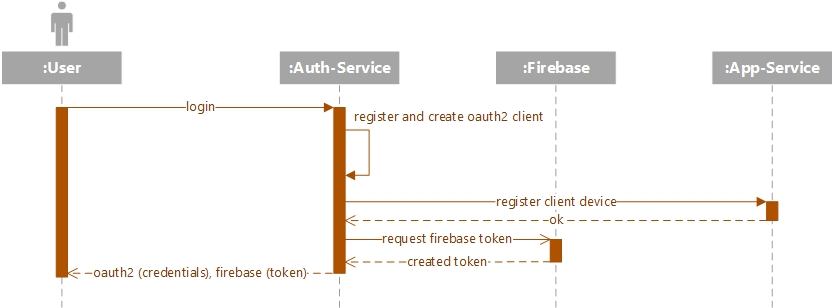
\includegraphics[scale=0.75]{\imageDir/sequence-client-login-auth-only.jpg}
	\caption{Sequenzdiagramm des Logins über einen mobilen \emph{Client}}
	\label{fig:image-sequence-client-login}
\end{figure}
\ \newline
Die Abbildung \ref{fig:image-sequence-client-login} zeigt den Ablauf des Logins eines Benutzers über einen mobilen \emph{Client}. Der Benutzer wird mit seinen Zugangsdaten via REST am \emph{Auth-Service} authentifiziert und es wird ein \emph{OAuth2-Client} für den verwendeten mobilen \emph{Client} erstellt, wobei die \emph{Client}-Anwendung einen eindeutigen Schlüssel für jedes Endgerät erzeugen muss. Dieser registrierte \emph{Client} wird an den \emph{App-Service} via REST übermittelt. Anschließend wird für den mobilen \emph{Client} auf \emph{Firebase} ein Token erstellt, mit dem sich der mobile \emph{Client} auf \emph{Firebase} authentifizieren kann. Als Antwort wird dem mobilen \emph{Client} folgendes JSON-Resultat übermittelt.
\newline
\begin{code}
	\caption{JSON-Antwort an den \emph{Client}}
	\jsonfile{\dataDir/client-login-json-response.json}
\end{code}
\ \newline
Das Registrieren des Clients vom \emph{Auth-Service} am \emph{App-Service} erfolgt über \emph{HTTP Basic Auth} geschützte Schnittstelle, die nur für einen Systembenutzer nutzbar ist, der dem \emph{Auth-Service} bekannt ist.

\subsubsection{\emph{Client} \emph{Firebase Cloud Messaging (FCM) Token} Registrierung}
Die Abbildung \ref{fig:image-sequence-fcm-token-registration} zeigt den Ablauf der Registrierung des FCM-Tokens am \emph{Auth-Service}, der wiederum vom \emph{Auth-Service} amd \emph{App-service} registriert wird. Die Registrierung über den \emph{Auth-Service} wurde gewählt, da dieser Service die Benutzer und deren Endgeräte verwaltet. Das Registrieren des FCM-Tokens am \emph{App-Service} erfolgt über eine \emph{HTTP BasicAuth} geschützte Schnittstelle, die nur für einen Systembenutzer nutzbar ist, der dem \emph{Auth-Service} bekannt ist. 
\newpage
\begin{figure}[h]
	\centering
	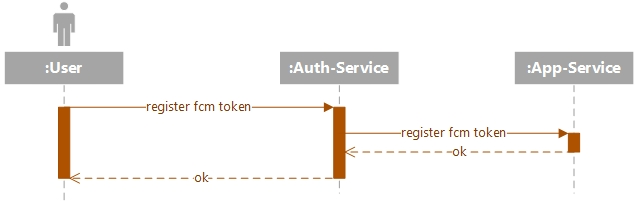
\includegraphics[scale=0.75]{\imageDir/fcm-token-registration}
	\caption{Sequenzdiagramm der Registrierung des FCM-Tokens}
	\label{fig:image-sequence-fcm-token-registration}
\end{figure}
\ \newline
Als Resultat wird bei dieser Schnittstelle nur der HTTP Statuscode 200 zurückgeliefert.

\subsection{\emph{Swagger Client} Generierung}
\label{sec:swagger-client-generation}
Dieser Abschnitt behandelt die Generierung der \emph{Clients} für die REST-Schnittstellen mit \emph{Swagger}. Das \emph{OpenSource}-Projekt \emph{SpringFox} stellt eine Integration von \emph{Swagger} für \emph{Spring MVC} zur Verfügung, mit der aus \emph{RestController} Implementierungen \emph{Swagger}-JSON-Definitionen erstellt werden können. Des Weiteren wird die \emph{Swagger-UI} mitgeliefert, mit der die implementierten REST-Schnittstellen getestet werden können.
\newline
\newline
Aus den generierten \emph{Swagger}-Definitionen der REST-Schnittstellen wurden \emph{Gradle} Projekte generiert, welche die implementierten \emph{Clients} enthalten. Die generierten Projekte wurden in das Wurzelprojekt \emph{java} mitaufgenommen, in dem sich alle Projekte des Projekts \emph{RPISec} befinden.
\newline
\newline
Für die Generierung wurden die beiden Skripte \emph{generate-clients.bat} und \emph{update-clients.bat} implementiert, wobei das Skript \emph{generate-clients.bat} die Projekte und \emph{Clients} generiert und das Skript \emph{update-clients.bat} nur die \emph{Clients} generiert. Damit die \emph{Client} Implementierungen generiert werden können, müssen die Services gestartet sein, da die \emph{Swagger}-JSON-Definitionen von \emph{SpringFox} nur beim Start der Anwendung generiert werden und nicht bei dessen \emph{Build}.
\newline
\newline
Die \emph{Swagger-UI} kann unter folgenden Link erreicht werden \emph{$<BASE\_URL>$/swagger-ui.html}, wobei die \emph{BASE\_URL} der Pfad ist, unter dem der \emph{Microservice} erreicht werden kann. Die \emph{BASE\_URL} hat das Format \emph{$<PROTOCOL>$://$<HOST>$:$<PORT>$/$<CONTEXT\_ROOT>$}. 
\newpage

\section{\emph{Docker} unterstützte Integrationstests}
Dieser Abschnitt behandelt die Integrationstests für die implementierten \emph{Microservices} in einer Docker Infrastruktur.
\begin{figure}[h]
	\centering
	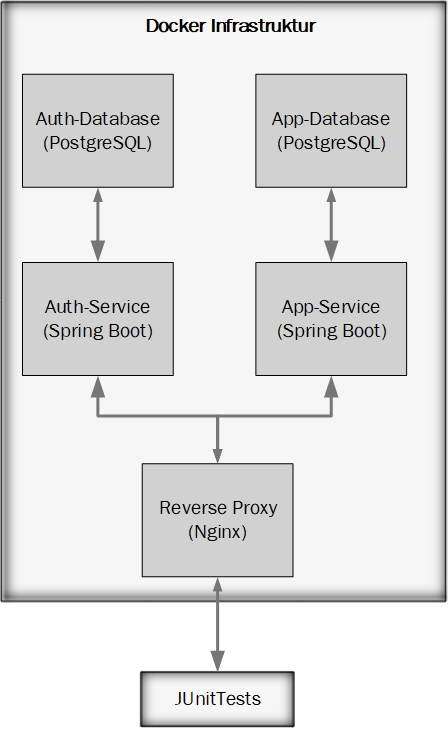
\includegraphics[scale=0.50]{\imageDir/integration-tests-docker-infrastructure}
	\caption{Aufbau der Integrationstests mit Docker Infrastruktur}
	\label{fig:integration-tests-docker-infrastructure}
\end{figure}
\ \newline
Die Abbildung \ref{fig:integration-tests-docker-infrastructure} zeigt den Aufbau der \emph{Docker} Infrastruktur und die Verbindung zu den implementierten \emph{JUnit}-Tests. Die Tests wurden in einer \emph{TestSuite} zusammengefasst, wobei diese Suite eine \emph{JUnit ClassRule} definiert, welche die \emph{Docker} Infrastruktur via \emph{Docker-Compose} vor der Ausführung der \emph{TestSuite} erstellt und startet und nach er Ausführung der \emph{TestSuite} die Infrastruktur stoppt und die \emph{Docker Container} entfernt. 
\newline
\newline
Es wurden jeweils zwei \emph{Dockerfiles} definiert \emph{Dockerfile-x86} und \emph{Dockerfile-pi}, welche ein \emph{Base Image} für die jeweilige Umgebung generieren. Die anderen \emph{Dockerfiles} leiten von dem \emph{Base Image rpisec-test-base} ab, das entweder über \emph{Dockerfile-x86} oder über \emph{Dockerfile-pi} erzeugt wurde, je nachdem auf welcher Umgebung die Tests ausgeführt werden sollen. Mit dem folgenden Befehl muss das \emph{Base Image} vor der Ausführung der Tests erzeugt werden.
\begin{minted}{bash}
docker build -t rpisec-test-base -f base/Dockerfile-[x86|pi] .
\end{minted}
Die verwendete \emph{JUnit ClassRule} wird von der Bibliothek \emph{docker-compose-rule-junit4}\footnote{\url{https://github.com/palantir/docker-compose-rule}} von \emph{Palantir} zur Verfügung gestellt, die es erlaubt über einen \emph{Builder} die \emph{ClassRule} zu konfigurieren und zu erstellen. Jedoch hat sich gezeigt, dass wenn während des Startens der \emph{Docker} Infrastruktur eine Ausnahme ausgelöst wird, die \emph{Docker} Infrastruktur nicht richtig runter gefahren wird und dadurch \emph{Docker Container} Namenskonflikte auftreten, die ein erneutes Starten der Tests verhindern.
\newline
\newline
Die Tests nutzen die im Abschnitt \ref{sec:swagger-client-generation} beschriebenen generierten \emph{Swagger Clients}, um die Kommunikation der \emph{Clients} mit den \emph{Auth-Service} zu testen. Es sei aber angemerkt dass es sich hier um reine \emph{Blackbox} Tests handelt, die nur aus der Sicht der \emph{Clients} testen.
\end{document}           
